% Converted from reference/DB4OFlare (MadCap Flare, Java target)

\chapter{Dependency Overview}
\label{ref:dependency-overview}

The different functionality of db4o is implemented in multiple jar s. You need to include only the jar which are required for you're application. Here's an overview:

\begin{center}
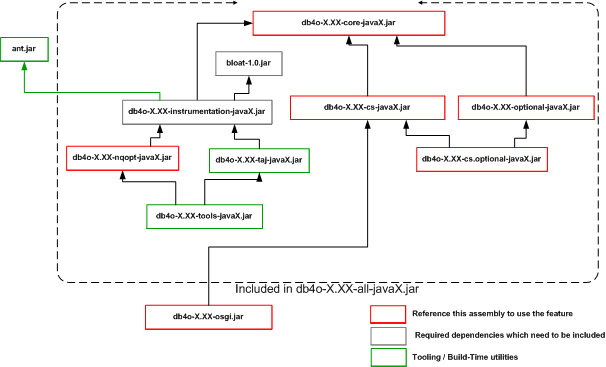
\includegraphics[width=\maxwidth]{images/ref-depedency-overview-java.png}
\end{center}
\section*{db4o-X.XX-core-javaX.jar}

This jar contains the \hyperref[ref:basics]{core functionality} (p.~\pageref{ref:basics}) of db4o. It doesn't have any dependencies to other jars.

\section*{db4o-X.XX-cs-javaX.jar}

This jar contains the \hyperref[ref:client-server]{client server mode} (p.~\pageref{ref:client-server}) of db4o. It only depends on the db4o-core jar.

\section*{db4o-X.XX-nqopt-javax.jar}

This jar contains the \hyperref[ref:basics-querying-native-queries]{native query optimizations} (p.~\pageref{ref:basics-querying-native-queries}) for db4o. Make sure that you include this jar when you use native queries. It depends on the db4o-core, db4o-instrumentation and the bloat jar for the runtime optimization.

When you use the \hyperref[ref:advanced-topics-enhancement-tools]{compile-time optimization} (p.~\pageref{ref:advanced-topics-enhancement-tools}) instead of the runtime optimization, it also requires the Ant library. However when you do compile-time optimization, you don't need this jar and its dependencies at runtime.

Note that the native queries work also without this jar in the classpath. However the queries cannot be optimized without this jar and will run a lot slower.

\section*{db4o-X.XX-optional-javaX.jar}

This jar contains some additional features and functionality for db4o, like \hyperref[ref:advanced-topics-runtime-statistics]{monitoring capabilities} (p.~\pageref{ref:advanced-topics-runtime-statistics}), \hyperref[ref:advanced-topics-type-handling-bigmath]{BigMath-support} (p.~\pageref{ref:advanced-topics-type-handling-bigmath}) and .NET support. It depends on the db4o-core jar.

\section*{db4o-X.XX-cs.optional-javaX.jar}

This jar contains additional features for the client-server-mode, like \hyperref[ref:client-server-pluggable-sockets-using-ssl-for-client-server-communication]{SSL} (p.~\pageref{ref:client-server-pluggable-sockets-using-ssl-for-client-server-communication}) and monitoring support. It depends on the db4o-cs, db4o-optional and the db4o-core jar.

\section*{db4o-X.XX-taj-javaX.jar}

This jar contains the utilities to enhance your classes with \hyperref[ref:advanced-topics-enhancement-tools]{transparent activation} (p.~\pageref{ref:advanced-topics-enhancement-tools}). It is normally used at compile time, but its possible to use it also at runtime. It depends on the db4o-core, db4o-instrumentation and the bloat-jar. Since the enhancement is usually done with Ant, it also requires the Ant-library.

\section*{db4o-X.XX-tools-javaX.jar}

This jar contains the \hyperref[ref:advanced-topics-enhancement-tools]{high level functionality for enhancing your classes} (p.~\pageref{ref:advanced-topics-enhancement-tools}). It requires the db4o-core, db4o-instrumentation, db4o-taj, db4o-nqopt and the bloat-jar. Additionally it needs the Ant-library.

\section*{db4o-X.XX-osgi.jar}

This jar contains a db4o OSGI service. It depends on the db4o-core and the db4o-cs jars.

\section*{db4o-X.XX-all-javaX.jar}

This jar contains all db4o functionality with all dependencies, except the Ant-library and the db4o-osgi library. If you just want to use db4o and aren't limited by space constrains use this jar only.

